%\documentclass{book}
\documentclass{report}

\pagenumbering{roman} 
\pagestyle{empty}

% Notas de aula
%
% Template criado em 24/9/2013
% Daniel Oliveira Dantas
%
% Ctrl+x 8 , c = ç

\usepackage[utf8]{inputenc}
\usepackage[english, brazil]{babel}

\usepackage{listings}
\lstset{
  language=C,                % choose the language of the code
  numbers=none,                   % where to put the line-numbers
  stepnumber=1,                   % the step between two line-numbers.        
  numbersep=10pt,                  % how far the line-numbers are from the code
  %backgroundcolor=\color{white},  % choose the background color. You must add \usepackage{color}
  showspaces=false,               % show spaces adding particular underscores
  showstringspaces=false,         % underline spaces within strings
  showtabs=false,                 % show tabs within strings adding particular underscores
  tabsize=2,                      % sets default tabsize to 2 spaces
  captionpos=b,                   % sets the caption-position to bottom
  breaklines=true,                % sets automatic line breaking
  breakatwhitespace=true,         % sets if automatic breaks should only happen at whitespace
  title=\lstname,                 % show the filename of files included with \lstinputlisting;
}

% Adicionado para permitir a criação de listas com vários graus de aninhamento
% ddantas, 24/03/2020
\usepackage{amssymb}
\usepackage{amsmath}
\usepackage[ampersand]{easylist}
\ListProperties(Hide=100, Hang=true, Progressive=3ex, Style*=--- ,
Style2*=$\bullet$ ,Style3*=$\circ$ ,Style4*=\tiny$\blacksquare$ )

% Adicionado para permitir a inserção de figuras
% ddantas, 24/03/2020
\usepackage{graphicx}

% Adicionado para permitir a inserção de figuras
% ddantas, 31/03/2020
\usepackage{subcaption}

%formatacao

\newcommand{\TAB}{{\hspace*{1cm}}}
\newcommand{\NEWLINE}{~\\}
\newcommand{\BV}{\begin{verbatim}}
\newcommand{\EV}{\end{verbatim}}

%tipos de dados

\newcommand{\VOID}{{\tt void}}
\newcommand{\CHAR}{{\tt char}}
\newcommand{\INT}{{\tt int}}
\newcommand{\FLOAT}{{\tt float}}
\newcommand{\DOUBLE}{{\tt double}}

\newcommand{\LONGINT}{{\tt long int}}

%operadores

\newcommand{\AND}{{\tt \&\&}}
\newcommand{\OR}{{\tt ||}}

\newcommand{\LNOT}{{\tt \~{}}}
\newcommand{\LAND}{{\tt \&}}
\newcommand{\LOR}{{\tt |}}
\newcommand{\LXOR}{{\tt \^{}}}

%palavras reservadas

\newcommand{\IF}{{\tt if}}
\newcommand{\ELSE}{{\tt else}}

\newcommand{\SWITCH}{{\tt switch}}
\newcommand{\CASE}{{\tt case}}

\newcommand{\FOR}{{\tt for}}
\newcommand{\WHILE}{{\tt while}}

\newcommand{\BREAK}{{\tt break}}

\newcommand{\TRUE}{{\tt true}}
\newcommand{\FALSE}{{\tt false}}

\newcommand{\MAIN}{{\tt main}}

\newcommand{\SIZEOF}{{\tt sizeof}}

% funcoes

\newcommand{\SIN}{{\tt sin}}
\newcommand{\COS}{{\tt cos}}
\newcommand{\TAN}{{\tt tan}}
\newcommand{\LOG}{{\tt log}}

\newcommand{\PRINTF}{{\tt printf}}
\newcommand{\SCANF}{{\tt scanf}}

\newcommand{\SPRINTF}{{\tt sprintf}}
\newcommand{\SSCANF}{{\tt sscanf}}

\newcommand{\FPRINTF}{{\tt fprintf}}
\newcommand{\FSCANF}{{\tt fscanf}}

\newcommand{\GETS}{{\tt gets}}
\newcommand{\FGETS}{{\tt fgets}}

\newcommand{\FOPEN}{{\tt fopen}}
\newcommand{\FCLOSE}{{\tt fclose}}

\newcommand{\SYSTEM}{{\tt system}}

% outros

\newcommand{\source}[1]{  \vspace{-6pt}  \caption*{ \footnotesize{Fonte: {#1}} }  }
\newcommand{\ind}{\hspace{1cm}}

%renewcommand

\renewcommand\chaptername{Capítulo}
\renewcommand\lstlistingname{Listagem}



\title{Notas de aula de Processamento de imagens e Visão Computacional}
\author{Daniel Oliveira Dantas}
\date{24 de março de 2020}
\begin{document}

\maketitle

%%%%%%%%%%%%%%%%%%%%%%%%%%%%%%%%%%%%%%%%%%%%%%%%%%%%%%%%%%%%
%Índice
%%%%%%%%%%%%%%%%%%%%%%%%%%%%%%%%%%%%%%%%%%%%%%%%%%%%%%%%%%%%

\tableofcontents
\pagestyle{plain}


%%%%%%%%%%%%%%%%%%%%%%%%%%%%%%%%%%%%%%%%%%%%%%%%%%%%%%%%%%%%
%Capítulo: Introdução
%%%%%%%%%%%%%%%%%%%%%%%%%%%%%%%%%%%%%%%%%%%%%%%%%%%%%%%%%%%%

\chapter{Introdução}


\setcounter{page}{1}    % set page to 1 again to start arabic count
\pagenumbering{arabic}


Capítulo 1 de Gonzalez, \textit{Digital Image Processing}~\cite{gonzalez2006image}.

%%%%%%%%%%%%%%%%%%%%%%%%%%%%%%%%%%%%%%%%%%%%%%%%%%%%%%%%%%%%
\section{O que é processamento de imagens}

\begin{easylist}
  & O que é uma imagem?
  && Uma matriz
  && Uma função
  && Esses conceitos podem ser generalizados para mais dimensões
  & Uma definição de processamento de imagens: processo em que tanto a entrada quanto a saída são imagens.
  && Essa definição não engloba, porém, processos como valor médio da imagem, extração de pontos característicos, alguns tipos de reconstrução 3D, aplicações de segurança que detectam atividades suspeitas, reconhecimento de gestos, reconhecimento de caracteres (OCR) e outras aplicações consideradas do campo de visão computacional.
  & Uma definição mais abrangente: processos de baixo, médio e alto nível em que tanto a entrada quanto a saída são imagens.
  && Baixo nível: envolve operações primitivas, de redução de ruído, aumento de contraste, aumento de nitidez (\textit{sharpening}), \textit{thresholding} etc. Nos processos de baixo nível, tanto a entrada quanto a saída são imagens.
  && Médio nível: envolve tarefas como segmentação (particionamento), redução dos objetos a uma descrição ou formato apropriado para processamento, classificação (reconhecimento) de objetos. A entrada são imagens, e a saída são atributos extraídos dessas imagens, como bordas, contornos, características ou classe de objetos individuais.
  && Alto nível: envolve atividades cognitivas associadas com a visão. Cognição envolve atividades como memória, compreensão, aprendizado, raciocínio, atenção, resolução de problemas e tomada de decisão.
\end{easylist}

%%%%%%%%%%%%%%%%%%%%%%%%%%%%%%%%%%%%%%%%%%%%%%%%%%%%%%%%%%%%
\section{Origens do processamento digital de imagens}

\begin{easylist}
  & 1920: \textit{Bartlane cable picture transmission system}, 5 tons de cinza.
  & 1929: idem, 15 tons de cinza.
  & 1948: invenção do transistor.
  & 1950 a 1960: invenção das linguagens de programação de alto nível, COBOL e Fortran.
  & 1958: invenção do circuito integrado.
  & 1964: primeira foto da Lua tirada de uma sonda.
  & 1968 a 1971: invenção dos primeiros microprocessadores, CADC, TMS1000, 4004.
  & 1969: invenção do CCD.
  & 1971: primeira tomografia computadorizada
\end{easylist}

%%%%%%%%%%%%%%%%%%%%%%%%%%%%%%%%%%%%%%%%%%%%%%%%%%%%%%%%%%%%
\section{Áreas que usam processamento digital de imagens}

\begin{easylist}
  & Medicina, astronomia, meteorologia, indústria, fotografia, editoração, segurança etc.
  & Técnicas de obtenção de imagem:
  && Eletromagnética: luz, radiação UV, radiação IR, raios X, raios gama, microondas.
  && Eletrônica: microscopia eletrônica.
  && Mecânica: ondas acústicas, ultrassom.
  && Sintética: computação gráfica, fractais.
\end{easylist}

%%%%%%%%%%%%%%%%%%%%%%%%%%%%%%%%%%%%%%%%%%%%%%%%%%%%%%%%%%%%
\section{Passos fundamentais no processamento digital de imagens}

\begin{easylist}
& Aquisição
& Melhoramento (\textit{image enhancement)}
& Restauração
& Processamento de cores
& \textit{Wavelets} e processamento multirresolução
& Compressão
& Processamento morfológico
& Segmentação
& Representação e descrição
& Reconhecimento de objetos
\end{easylist}


%%%%%%%%%%%%%%%%%%%%%%%%%%%%%%%%%%%%%%%%%%%%%%%%%%%%%%%%%%%%
\section{Componentes de um sistema de processamento de imagens}

\begin{easylist}
& Sensores + \textit{hardware} especializado
& Computador + GPU
& Armazenamento em massa
& \textit{Software} de processamento de imagens
& Monitor de imagem
& Impressora
& Rede
\end{easylist}



%%%%%%%%%%%%%%%%%%%%%%%%%%%%%%%%%%%%%%%%%%%%%%%%%%%%%%%%%%%%
%Capítulo: Fundamentos de imagens digitais
%%%%%%%%%%%%%%%%%%%%%%%%%%%%%%%%%%%%%%%%%%%%%%%%%%%%%%%%%%%%

\chapter{Fundamentos de imagens digitais}

Capítulo 2 de Gonzalez, \textit{Digital Image Processing}~\cite{gonzalez2006image}.

%%%%%%%%%%%%%%%%%%%%%%%%%%%%%%%%%%%%%%%%%%%%%%%%%%%%%%%%%%%%
\section{Elementos de percepção visual}

%%%%%%%%%%%%%%%%%%%%%%%%%%%%%%%%%%%%%%%%%%%%%%%%%%%%%%%%%%%%
\section{Luz e o espectro eletromagnético}

\begin{easylist}
& Frequência: $f$.
& Comprimento de onda: $\lambda$.
& Velocidade da luz: $ c = 3 \times 10^8 \text{m/s}, c=\lambda f$.
& Constante de Planck: $ h = 6.6 \times 10^{-34} \text{Js (m$^2$kg/s)} $, $E = hf$.
\end{easylist}



\begin{figure}[!h]
  \begin{center}
    \begin{tabular}{c}
      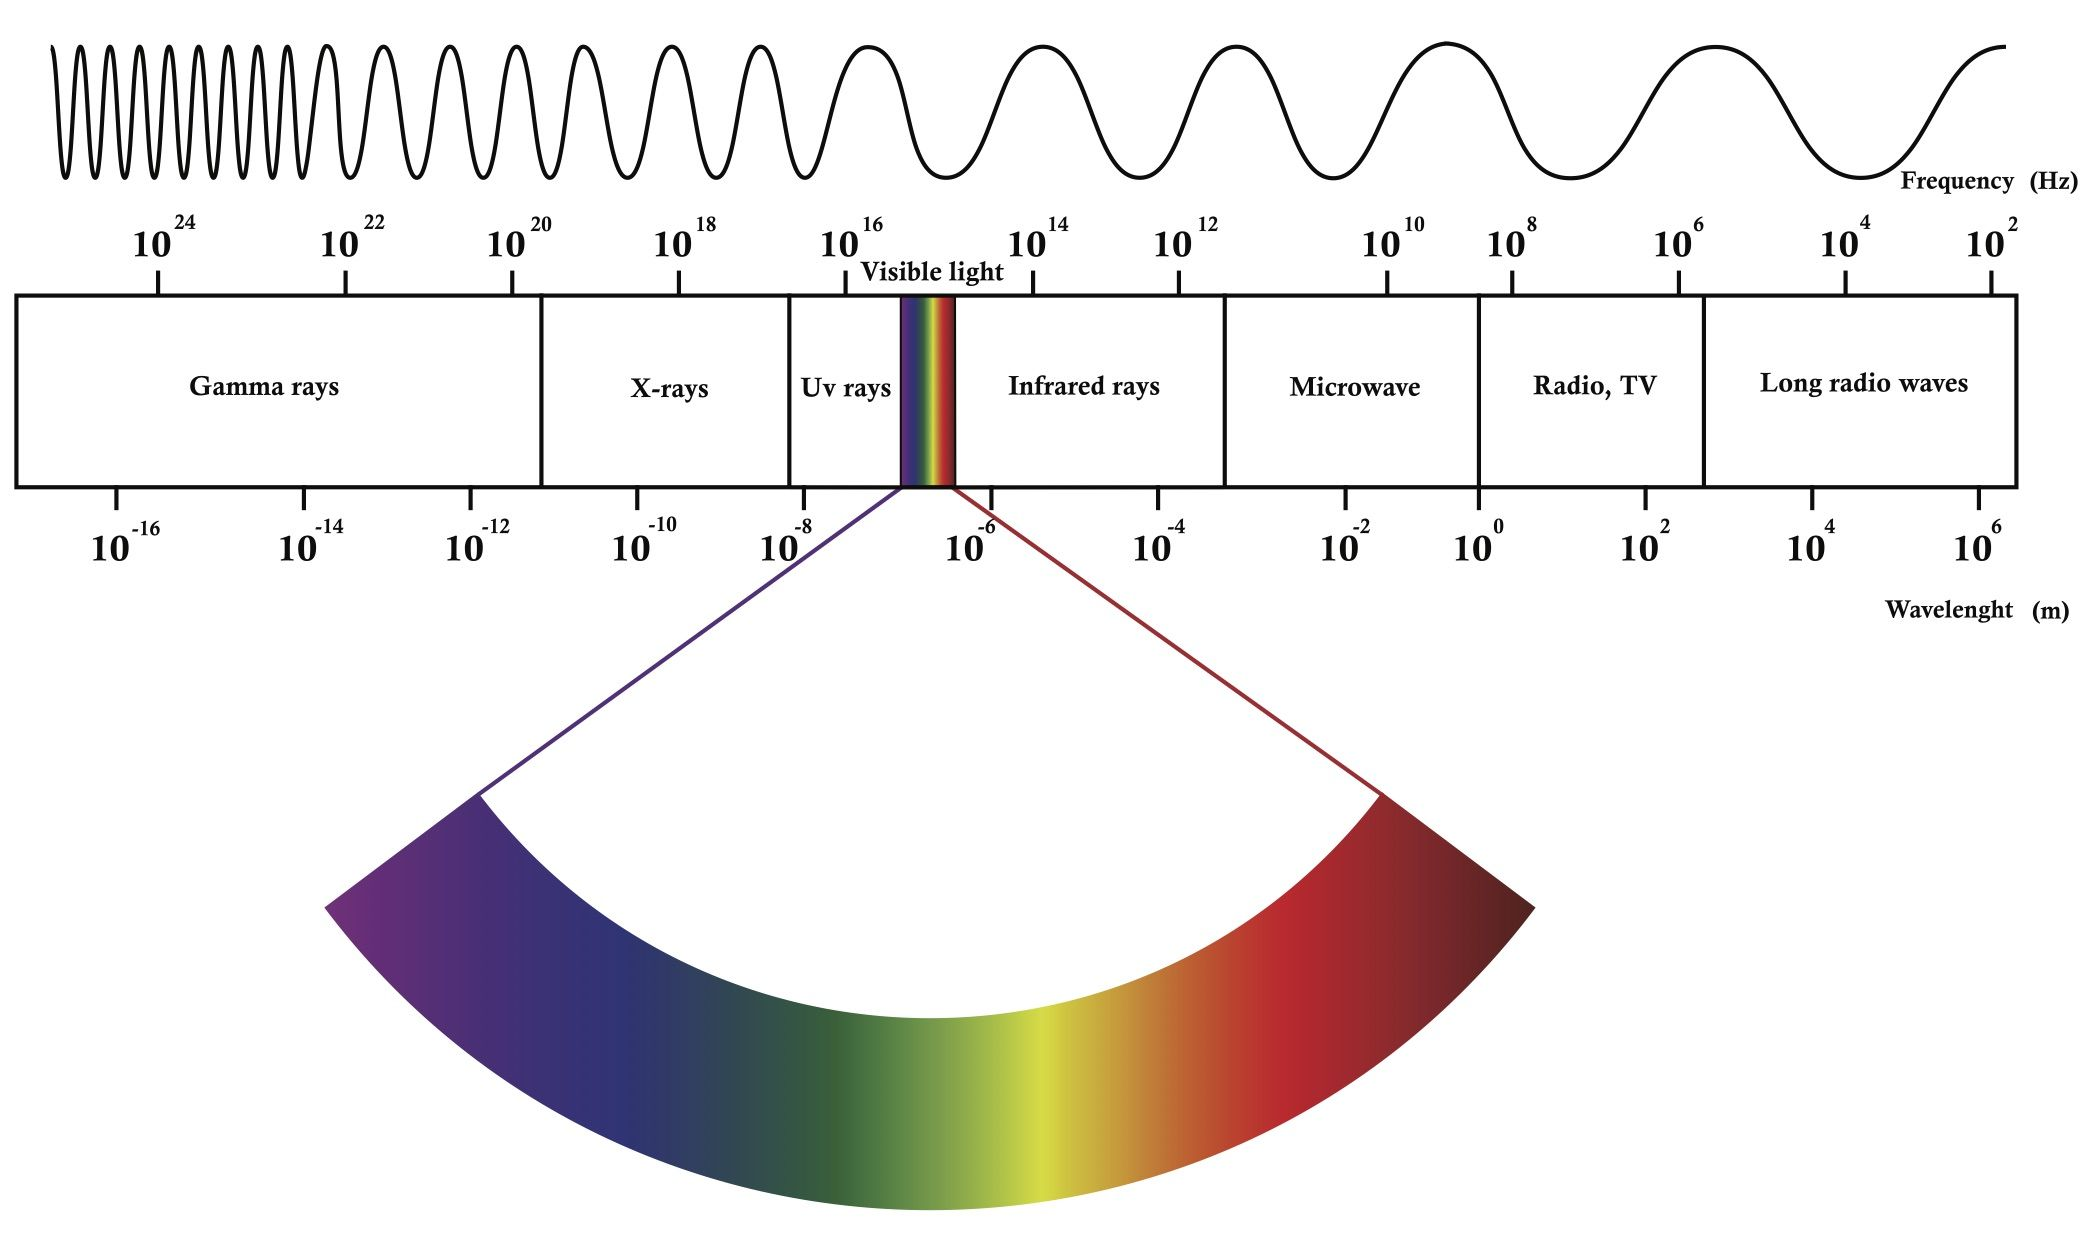
\includegraphics[width=0.7\textwidth]{images/02/spectrum.png}
    \end{tabular}
  \end{center}
  \caption{\label{fig:spectrum} Espectro eletromagnético}
  \source{\tt{https://www.livescience.com/38169-electromagnetism.html}.}
\end{figure}


%%%%%%%%%%%%%%%%%%%%%%%%%%%%%%%%%%%%%%%%%%%%%%%%%%%%%%%%%%%%
\section{Aquisição de imagens}

\begin{easylist}
& Normalmente é feita através de componentes sensíveis a alguma faixa específica do espectro eletromagnético
&& Sensores simples: fotodiodo, fototransistor.
&& Sensores lineares: CCD linear.
&& Sensores em matriz: CCD de câmeras fotográficas, mouse ótico.
\end{easylist}

\begin{figure}[!h]
  \begin{center}
    \begin{tabular}{c}
      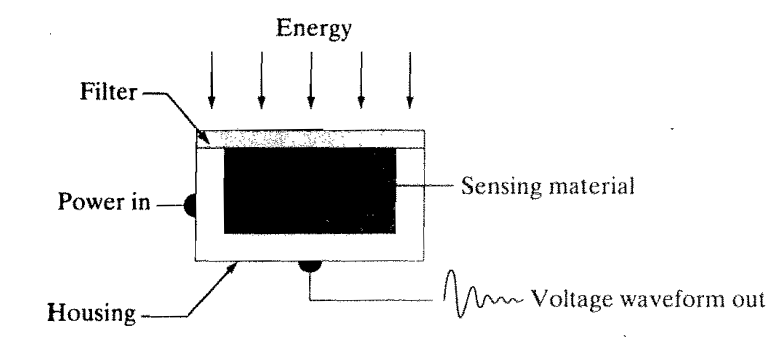
\includegraphics[width=0.8\textwidth]{images/02/sensor.png}
    \end{tabular}
  \end{center}
  \caption{\label{fig:sensor} Esquema de um sensor}
  \source{Gonzalez~\cite{gonzalez2006image}.}
\end{figure}


%%%%%%%%%%%%%%%%%%%%%%%%%%%%%%%%%%%%%%%%%%%%%%%%%%%%%%%%%%%%
\section{Amostragem e quantização}

\begin{easylist}
& Amostragem: digitalização dos valores das coordenadas, tanto no espaço quanto no tempo.
& Quantização: digitalização dos valores das amplitudes
& Representação: 
&& Matriz
\end{easylist}

  \begin{equation*}
    f(i, j) =
    \begin{bmatrix}
      f(0, 0)   & f(0, 1)   & \dots  & f(0, N-1)   \\
      f(1, 0)   & f(1, 1)   & \dots  & f(1, N-1)   \\
      \vdots    & \vdots    & \ddots & \vdots      \\
      f(M-1, 0) & f(M-1, 1) & \dots  & f(M-1, N-1) 
    \end{bmatrix}      
  \end{equation*}
    
\begin{easylist}
&& Função
\end{easylist}
  
  \begin{align*}
    & f: \mathbb{Z}^2 \rightarrow \mathbb{Z} \\
    & f: \{0, \dots, M-1\} \times \{0, \dots, N-1\} \rightarrow \{0, \dots, L-1\}
  \end{align*}

\noindent
onde $L = 2^k$. $L$ é o intervalo dinâmico do sensor e $k$ é o número de bits necessários para representar $L$.

\vspace{1cm}
  
\begin{easylist}
&& Número de bits necessários para armazenar uma imagem $M \times N$:  
\end{easylist}

\[
  b = MNk  
\]

\begin{easylist}
&& Número de bytes necessários para armazenar uma imagem $M \times N$:  
\end{easylist}

\[
  B = MNk/8  
\]



\begin{easylist}
& Redimensionamento de imagem: \textit{zoom} ou \textit{resize}
&& \textit{Nearest neighbor}: ampliar uma imagem replicando cada pixel várias vezes.
&& Bilinear: ampliar uma imagem inserindo pixels calculados da interpolação linear entre os pixels mais próximos.
\end{easylist}

%%%%%%%%%%%%%%%%%%%%%%%%%%%%%%%%%%%%%%%%%%%%%%%%%%%%%%%%%%%%
\section{Relações entre pixels}

\begin{easylist}
& Adjacência: é uma relação entre dois poxels com as propriedades listadas abaixo.
\end{easylist}

  \begin{align*}
    & 1.\; A(p, q) \Leftrightarrow x \neq y  && \text{irreflexiva} \\
    & 2.\; A(p, q) \Leftrightarrow A(q, p)   && \text{simétrica} \\
  \end{align*}
 
\begin{easylist}
&& 4-adjacência: os vizinhos de $(x, y)$ são $(x, y-1)$, $(x, y+1)$, $(x-1, y)$ e $(x+1, y)$.
&& D-adjacência: os vizinhos de $(x, y)$ são $(x-1, y-1)$, $(x-1, y+1)$, $(x+1, y+1)$ e $(x+1, y-1)$.
&& 8-adjacência: os vizinhos de $(x, y)$ são a união da 4-adjacência e da D-adjacência.
\end{easylist}

\vspace{1cm}

\begin{table}[!h]
  \centering
  \begin{tabular}{|c|c|c|}
        \hline
        $(x-1, y-1)$ & $(x, y-1)$ & $(x+1, y-1)$ \\
        \hline
        $(x-1, y  )$ & $(x, y  )$ & $(x+1, y  )$ \\
        \hline
        $(x-1, y+1)$ & $(x, y+1)$ & $(x+1, y+1)$ \\
        \hline
  \end{tabular}
  \caption{Disposição dos pixels na vizinhança de $(x, y)$.}
\end{table}


\begin{easylist}
& Distância: sejam $p$ e $q$ dois pixels pertencentes a $P$, uma distância é uma função $D:P\times P \rightarrow \mathbb{R}$ com as propriedades listadas abaixo.  
\end{easylist}

  \begin{align*}
    & 1.\; D(p, q) \geq 0 \\
    & 2.\; D(p, q) = 0 \Leftrightarrow p = q \\
    & 3.\; D(p, q) = D(q, p)                 && \text{simetria} \\
    & 4.\; D(p, q) \leq D(p, z) + D(z, q)    && \text{desigualdade triangular}    \\
  \end{align*}

\begin{easylist}
&& Distância Euclidiana:           $D_e(p, q) = \sqrt{(p_x - q_x)^2 + (p_y - q_y)^2}$
&& Distância \textit{city-block}:  $D_4(p, q) = |p_x - q_x| + |p_y - q_y|$
&& Distância \textit{chessboard}:  $D_8(p, q) = \max(|p_x - q_x|, |p_y - q_y|)$
\end{easylist}


%%%%%%%%%%%%%%%%%%%%%%%%%%%%%%%%%%%%%%%%%%%%%%%%%%%%%%%%%%%%
\section{Ferramentas matemáticas}

\begin{easylist}
& Operações lineares: seja $H$ uma operação cuja entrada e saída são imagens, sejam $f$ e $g$ duas imagens, e $a$ e $b$, dois escalares. A operação $H$ é dita linear se segue a relação abaixo

  \[
    H(af + bg) = aH(f) + bH(g)
  \]

& Operações não-lineares: uma operação é dita não-linear se não é linear.
\end{easylist}




%%%%%%%%%%%%%%%%%%%%%%%%%%%%%%%%%%%%%%%%%%%%%%%%%%%%%%%%%%%%
%Capítulo: Image enhancement
%%%%%%%%%%%%%%%%%%%%%%%%%%%%%%%%%%%%%%%%%%%%%%%%%%%%%%%%%%%%

\chapter{\emph{Image Enhancement} (melhoramento) no domínio do espaço}

Capítulo 3 de Gonzalez, \textit{Digital Image Processing}~\cite{gonzalez2006image}.

%%%%%%%%%%%%%%%%%%%%%%%%%%%%%%%%%%%%%%%%%%%%%%%%%%%%%%%%%%%%
\section{Introdução}

\begin{easylist}
  & Métodos que operam no domínio do espaço podem ser denotados pela fórmula
  \[ g(x, y) = T(f(x, y)) \]

  onde $g(x, y)$ é a imagem de saída, $f(x, y)$ é a imagem de entrada, e $T$ é uma operação sobre $f$, definida sobre alguma vizinhança de $(x, y)$. $T$ pode operar sobre uma imagem ou um conjunto de imagens de entrada.
 
  & A forma mais simples de $T$ é quando a vizinhança tem tamanho $1\times 1$, ou seja, um único pixel. Nesse caso, $T$ é chamado \textit{gray-level transformation function}, ou \textit{intensity} ou \textit{mapping transformation function}, da forma
  \[ s = T(r) \]

  onde $s$ denota a intensidade de $g(x, y)$, e $r$, a intensidade de $f(x, y)$ em qualquer ponto $(x, y)$.

  && Um exemplo de transformação para aumentar o contraste da imagem de entrada pode ser visto na Figura~\ref{fig:contrast}.


  && \textit{Thresholding}: é como a transformação anterior levada ao extremo. Também aumenta o contraste, e a imagem de saída fica com apenas duas intensidades. Um exemplo dessa transformação pode ser visto na Figura~\ref{fig:thresh}.

\end{easylist}

\clearpage


\begin{figure}[!h]
  \begin{subfigure}{.5\textwidth}
    \centering
    \begin{tabular}{c}
      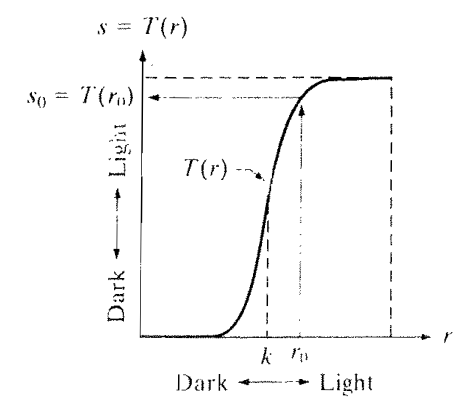
\includegraphics[width=1\textwidth]{images/03/01.png}
    \end{tabular}
    \caption{\label{fig:contrast} Aumento de contraste}
  \end{subfigure}
  \begin{subfigure}{.5\textwidth}
    \centering
    \begin{tabular}{c}
      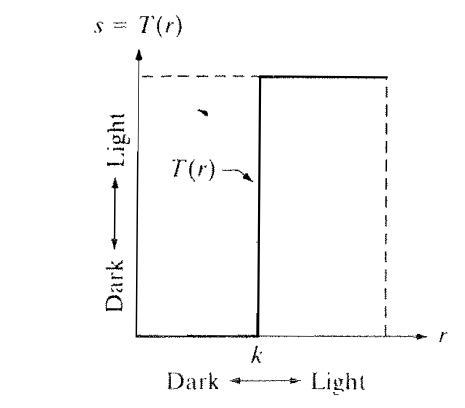
\includegraphics[width=1\textwidth]{images/03/02.png}
    \end{tabular}
    \caption{\label{fig:thresh} \textit{Threshold}}
  \end{subfigure}
  \caption{\label{fig:gray} \textit{Gray-level transformations}}
  \source{Gonzalez~\cite{gonzalez2006image}.}
\end{figure}


%%%%%%%%%%%%%%%%%%%%%%%%%%%%%%%%%%%%%%%%%%%%%%%%%%%%%%%%%%%%
\section{\emph{Gray-level transformations} simples}

\begin{easylist}

  & Negação: ver Figura~\ref{fig:gray2}.
  \[ s = L-1-r \]
  & Transformações logarítmicas: ver Figura~\ref{fig:gray2}.
  \[ s = c \log(1+r) \]
  & Transformações por potenciação: ver Figura~\ref{fig:power}.
  \[ s = cr^\gamma \]
  & \textit{Piecewise linear transformations}: ver Figura~\ref{fig:piece}.

\end{easylist}

\begin{figure}[!h]
  \begin{center}
    \begin{tabular}{c}
      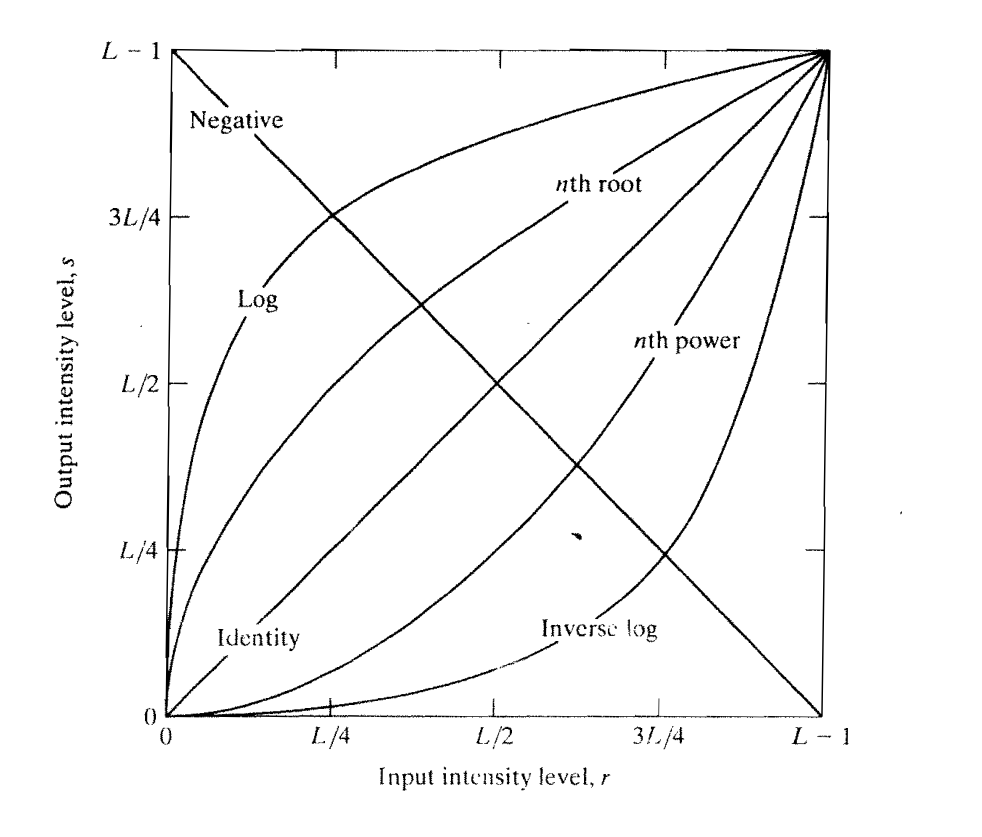
\includegraphics[width=0.70\textwidth]{images/03/03.png}
    \end{tabular}
  \end{center}
  \caption{\label{fig:gray2} Exemplos de \textit{gray-level transformations} simples.}
  %\source{Gonzalez~\cite{gonzalez2006image}.}
\end{figure}

\begin{figure}[!h]
  \begin{center}
    \begin{tabular}{c}
      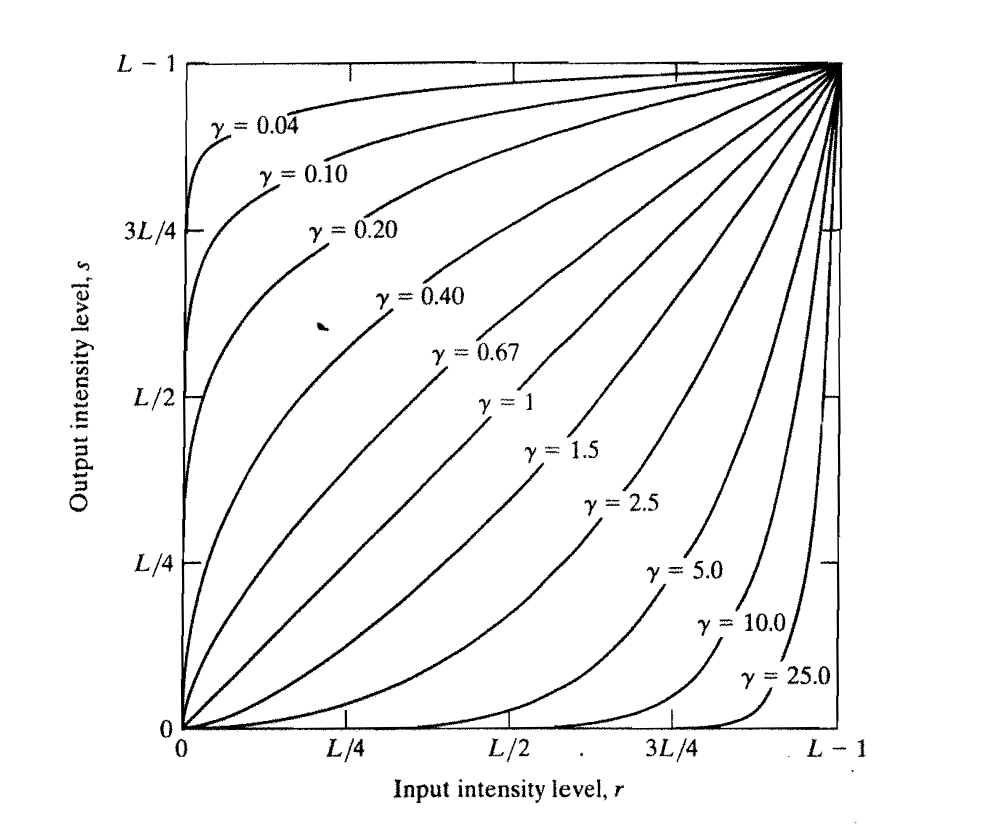
\includegraphics[width=0.70\textwidth]{images/03/04.png}
    \end{tabular}
  \end{center}
  \caption{\label{fig:power} Transformações por potenciação com diferentes expoentes}
  \source{Gonzalez~\cite{gonzalez2006image}.}
\end{figure}

\clearpage

\begin{figure}[!h]
  \begin{center}
    \begin{tabular}{c}
      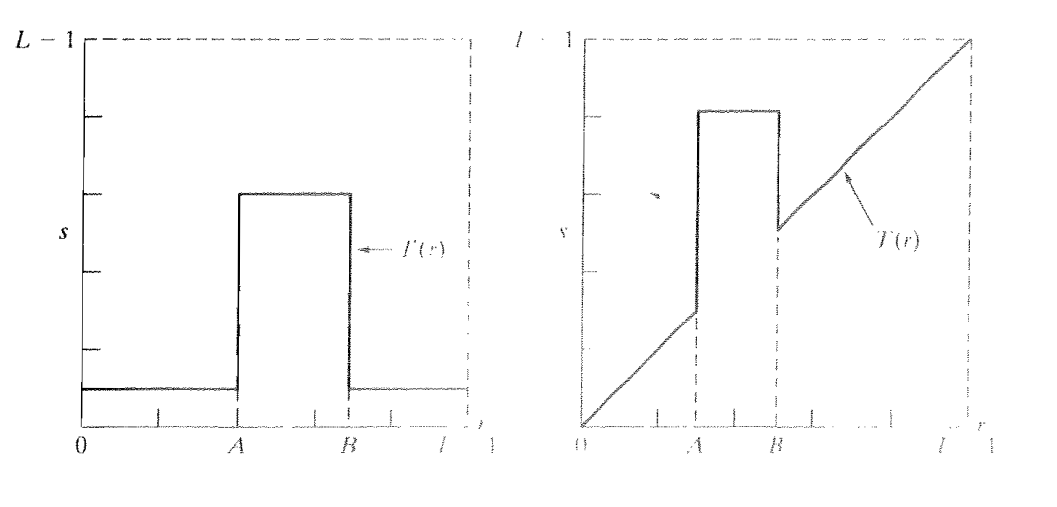
\includegraphics[width=0.9\textwidth]{images/03/05.png}
    \end{tabular}
  \end{center}
  \caption{\label{fig:piece} \textit{Piecewise linear transformations}}
  \source{Gonzalez~\cite{gonzalez2006image}.}
\end{figure}


%%%%%%%%%%%%%%%%%%%%%%%%%%%%%%%%%%%%%%%%%%%%%%%%%%%%%%%%%%%%
\section{Processamento de histograma}

\begin{easylist}

  & Histograma: de uma imagem digital com tons de cinza no intervalo $[0, L-1]$ é uma função discreta $h(r_k) = n_k$, onde $k$ é o $k$-ésimo tom de cinza, $r_k = k / (L-1)$ e $n_k$ é o número de pixels na imagem com tom de cinza igual a $k$.

  & Histograma normalizado: é dado por $p(r_k) = n_k / n$, onde $n$ é o total de pixels da imagem.

  & Equalização de histograma: é uma transformação que distribui uniformemente as escalas de cinza pelo intervalo dinâmico.

  \[ s = T(r), 0 \leq r \leq 1 \].

  && T(r) tem valor único e é monotonicamente crescente no intervalo $0 \leq r \leq 1$.

  && $0 \leq T(r) \leq 1$ para $0 \leq r \leq 1$.

  A probabilidade de ocorrência de um tom de cinza na imagem é

  \[ p(r_k) = n_k / n, k \in [0, L-1] \]

  \[ T(r_k) = \sum_{j=0}^k p(r_j) = \sum_{j=0}^k \frac {n_j}{n} \]
  
\end{easylist}


%%%%%%%%%%%%%%%%%%%%%%%%%%%%%%%%%%%%%%%%%%%%%%%%%%%%%%%%%%%%
\section{Operações aritméticas e lógicas}

\begin{easylist}

  & Interseção ou \textit{AND} lógico ou mínimo entre duas imagens: útil para aplicar máscaras.

  & Subtração: útil em imagens médicas com contraste radioativo.

  & Média: útil para diminuir o ruído quando é possível tirar várias fotos de um mesmo ponto de vista. Aplicada em astronomia.
  
\end{easylist}


%%%%%%%%%%%%%%%%%%%%%%%%%%%%%%%%%%%%%%%%%%%%%%%%%%%%%%%%%%%%
\section{Filtragem espacial}

\begin{easylist}

  & Filtragem espacial linear: é dada pela soma de pixels multiplicados por pesos
  && Correlação:

  \[ g(x, y) = \sum_{s = -a}^a\sum_{t = -b}^b w(s, t) f(x+s, y+t) \]

  onde $g$ é a imagem de saída, $(2a+1)(2b+1)$ é o tamanho do filtro, máscara, \textit{kernel} ou janela, e $f$ é a imagem de entrada.
  
  && Convolução:

  \[ g(x, y) = \sum_{s = -a}^a\sum_{t = -b}^b w(s, t) f(x-s, y-t) \]

  & Filtragem espacial não-linear: mediana, variância, filtros morfológicos dentre outros.
  
\end{easylist}


%%%%%%%%%%%%%%%%%%%%%%%%%%%%%%%%%%%%%%%%%%%%%%%%%%%%%%%%%%%%
\section{Suavização}

\begin{easylist}

  & Filtro de média:

\end{easylist}

  \[ \frac 1 9
    \begin{bmatrix}
      1 & 1 & 1 \\
      1 & 1 & 1 \\
      1 & 1 & 1 \\
    \end{bmatrix}  
  \]

\begin{easylist}

  & Filtro Gaussiano ou suavização Gaussiana ou \textit{blur}:

\end{easylist}

  \[ \frac 1 {16}
    \begin{bmatrix}
      1 & 2 & 1 \\
      2 & 4 & 2 \\
      1 & 2 & 1 \\
    \end{bmatrix}  
  \]

  \[ \frac 1 4
    \begin{bmatrix}
      1 & 2 & 1 \\
    \end{bmatrix}  
  \]
  \[ \frac 1 4
    \begin{bmatrix}
      1 \\
      2 \\
      1 \\
    \end{bmatrix}  
  \]
  
\begin{easylist}

  & Filtro de estatísticas de ordem: mediana, máximo, mínimo etc.

\end{easylist}


%%%%%%%%%%%%%%%%%%%%%%%%%%%%%%%%%%%%%%%%%%%%%%%%%%%%%%%%%%%%
\section{\emph{Sharpening}}

\begin{easylist}

  & Derivada de primeira ordem:

  \[ \frac {\partial f}{\partial x} = \frac {df}{dx} = f(x+1) - f(x) \]

  & Derivada de segunda ordem:

  \[ \frac {\partial^2 f}{\partial x^2} = f(x+1)  + f(x-1) - 2f(x) \]

  & Laplaciano:

  \[ \nabla^2 f = \frac {\partial^2 f}{\partial x^2} + \frac {\partial^2 f}{\partial y^2} \]

  \[ \frac {\partial^2 f}{\partial x^2} = f(x+1, y) + f(x-1, y) - 2f(x, y) \]

  \[ \frac {\partial^2 f}{\partial y^2} = f(x, y+1) + f(x, y-1) - 2f(x, y) \]

  \[ \nabla^2 f = f(x+1, y) + f(x-1, y) + f(x, y+1) + f(x, y-1) - 4f(x, y) \]

  & \textit{Sharpening}:

  \[ g(x, y) = f(x, y) - \nabla^2 f \]

\end{easylist}

  \[
    \begin{bmatrix}
       0 & -1 &  0 \\
      -1 &  5 & -1 \\
       0 & -1 &  0 \\
    \end{bmatrix}  
  \]

\begin{easylist}

  & \textit{Unsharp mask}:

  \[ g(x, y) = (1+\alpha) f(x, y) - \alpha \overline f (x, y), \alpha \in [0.0, 1.0] \]

  onde $\overline f (x, y)$ denota a imagem $f (x, y)$ após uma operação de \textit{blur}.

  & O uso do gradiente:
  && Gradiente de um campo escalar é um campo vetorial que aponta para a direção de sua maior taxa de crescimento. Sua magnitude é a taxa de crescimento.

  \[ \nabla f =
    \begin{bmatrix}
      \frac {\partial f}{\partial x} \\
      \frac {\partial f}{\partial y} \\
    \end{bmatrix}  
  \]

\clearpage
  
  && A magnitude do gradiente é dada por

  \[ \operatorname{mag}(\nabla f) = \sqrt{
      \left(\frac {\partial f}{\partial x}\right)^2 +
      \left(\frac {\partial f}{\partial y}\right)^2 }
  \]

  mas na prática, para evitar os quadrados e a raiz quadrada, se usa apenas 

  \[ \operatorname{mag}(\nabla f) =
      \left|\frac {\partial f}{\partial x}\right| +
      \left|\frac {\partial f}{\partial y}\right|
  \]

  && Considere a vizinhança a seguir:

\end{easylist}

\begin{table}[!h]
  \centering
  \begin{tabular}{|c|c|c|}
        \hline
        $p_1$ & $p_2$ & $p_3$ \\
        \hline
        $p_4$ & $p_5$ & $p_6$ \\
        \hline
        $p_7$ & $p_8$ & $p_9$ \\
        \hline
  \end{tabular}
  %\caption{Disposição dos pixels na vizinhança de $(x, y)$.}
\end{table}

\begin{easylist}

  O exmplo mais simples de cálculo do gradiente é

  \[ \operatorname{mag}(\nabla f) = |p_6 - p_5| + |p_8 - p_5| \]

  && \textit{Robert's cross gradient operator}:

  \[ \operatorname{mag}(\nabla f) = \sqrt{(p_9 - p_5)^2 + (p_8 - p_6)^2} \]
  
  ou, para simplificar,
  
  \[ \operatorname{mag}(\nabla f) = |p_9 - p_5| + |p_8 - p_6| \]
  
\end{easylist}
  



  




%%%%%%%%%%%%%%%%%%%%%%%%%%%%%%%%%%%%%%%%%%%%%%%%%%%%%%%%%%%%
%Capítulo: Image enhancement no domínio da frequência
%%%%%%%%%%%%%%%%%%%%%%%%%%%%%%%%%%%%%%%%%%%%%%%%%%%%%%%%%%%%

\chapter{\emph{Image Enhancement} (melhoramento) no domínio da frequência}

Capítulo 4 de Gonzalez, \textit{Digital Image Processing}~\cite{gonzalez2006image}.

\noindent
Seção 7 de Ramirez, \textit{The FFT: Fundamentals and Concepts}~\cite{ramirez1975fft}.

%%%%%%%%%%%%%%%%%%%%%%%%%%%%%%%%%%%%%%%%%%%%%%%%%%%%%%%%%%%%
\section{Introdução}

\begin{easylist}

  & Transformada de Fourier é uma maneira de representar um sinal como uma integral de senos e cossenos multiplicados por uma função de peso. Um sinal pode ser convertido para sua representação transformada e reconvertido de volta para o domínio original sem perda de informação. Também é possível realizar operações como filtragens na representação transformada e reconverter de volta para o domínio original.

\end{easylist}
  
%%%%%%%%%%%%%%%%%%%%%%%%%%%%%%%%%%%%%%%%%%%%%%%%%%%%%%%%%%%%
\section{A transformada de Fourier}

\begin{easylist}

  & Transformada de Fourier $g(u)$ de uma função contínua de uma única variável é dada pela fórmula

  \[ g(u) = \int^{\infty}_{-\infty} f(x) e^{-j2\pi ux} dx \]

  onde $j = \sqrt{-1}$, De maneira análoga, dado $g(u)$, podemos obter $f(x)$ através da transformada inversa de Fourier
  
  \[ f(x) = \int^{\infty}_{-\infty} g(u) e^{ j2\pi ux} du \]

\vspace{1cm}
  
  & Essas operações possuem uma versão para duas variáveis

  \[ g(u, v) = \int^{\infty}_{-\infty}\int^{\infty}_{-\infty} f(x, y) e^{-j2\pi (ux + vy)} dx dy \]

  e sua inversa

  \[ f(x, y) = \int^{\infty}_{-\infty}\int^{\infty}_{-\infty} g(u, v) e^{ j2\pi (ux + vy)} dx dy \]

  & Muitas vezes é mais fácil manipular as versões contínuas da transformada de Fourier, mas para trabalhar com imagens, usamos suas versões discretas

  \[ g(u) = \frac 1M \sum^{M-1}_{x=0} f(x) e^{-j2\pi ux/M} \textrm{para u de 0 a $M-1$} \]

  e sua inversa

  \[ f(x) =          \sum^{M-1}_{u=0} g(u) e^{ j2\pi ux/M} \textrm{para x de 0 a $M-1$} \]

  & O conceito de domínio da frequência segue a fórmula de Euler

  \[ e^{j\theta} = \cos\theta + j\sin\theta \]

  & Substituindo na transformada direta discreta, temos

  \[ g(u) = \frac 1M \sum^{M-1}_{x=0} f(x) (\cos (2\pi ux/M) -j\sin (2\pi ux/M)) \]

  & e na transformada inversa discreta, temos

  \[ f(x) = \sum^{M-1}_{u=0} g(u) (\cos (2\pi ux/M) +j\sin (2\pi ux/M)) \]

  & A transformada de Fourier discreta bidimensional pode ser calculada pela fórmula

  \[ g(u, v) = \frac 1{MN} \sum^{M-1}_{x=0}\sum^{N-1}_{y=0} f(x, y) e^{-j2\pi (ux/M + vy/N)} \].

  Nesse caso, a inversa pode ser calculada pela fórmula

  \[ f(x, y) =             \sum^{M-1}_{x=0}\sum^{N-1}_{y=0} g(u, v) e^{ j2\pi (ux/M + vy/N)} \].

\clearpage
  
  & Substituindo a fórmula de Euler na transformada discreta bidimensional de Fourier, obtemos

  \[ g(u, v) = \frac 1{MN} \sum^{M-1}_{x=0}\sum^{N-1}_{y=0} f(x, y)
      \cos\left(2\pi \left(\frac{ux}{M} + \frac{vy}{N}\right)\right) -
     j\sin\left(2\pi \left(\frac{ux}{M} + \frac{vy}{N}\right)\right)   \]

  e sua inversa

  \[ f(x, y) =             \sum^{M-1}_{x=0}\sum^{N-1}_{y=0} g(u, v)
      \cos\left(2\pi \left(\frac{ux}{M} + \frac{vy}{N}\right)\right) +
     j\sin\left(2\pi \left(\frac{ux}{M} + \frac{vy}{N}\right)\right)   \]

\end{easylist}
  
%%%%%%%%%%%%%%%%%%%%%%%%%%%%%%%%%%%%%%%%%%%%%%%%%%%%%%%%%%%%
\section{\textit{Fast Fourier Transform}}

\begin{easylist}

  & A complexidade do algoritmo da transformada de Fourier é quadrática no número de pixels da imagem. Para calcular cada pixel da imagem de saída, é necessário consultar todos os pixels da imagem de entrada. Se $P$ é o número de pixels da imagem, a complexidade da transformada de Fourier é $O(P^2)$. Felizmente, é possível acelerar o cálculo através do uso da Fast Fourier Transform (FFT), cuja complexidade é $O(P\log(P))$. A seguir veremos o algoritmo de Sande-Tukey descrito por Ramirez~\cite{ramirez1975fft}.

  & O algoritmo requer como entrada um vetor unidimensional cujo tamanho é uma potência de 2. Para processar imagens bidimensionais, é necessário primeiro aplicar o algoritmo em todas as linhas da imagem de entrada, e em seguida, em todas as colunas da imagem resultante.

  & A expressão para calcular a DFT de um sinal unidimensional é dada por

  \[ g(u) = \frac 1M \sum^{M-1}_{x=0} f(x) e^{-j2\pi ux/M} \]

para u de 0 a $M-1$.
  
  & Seja $W = e^{-j2\pi/M}$. Omitindo o fator $1/M$, que pode ser aplicado no final do cálculo, e trocando $f$ por $f_0$, onde o índice subscrito denota o estágio do cálculo, teremos

  \[ g(u) = \sum^{M-1}_{x=0} f_0(x) W^{-ux} \].

\begin{figure}[!b]
  \begin{center}
    \begin{tabular}{c}
      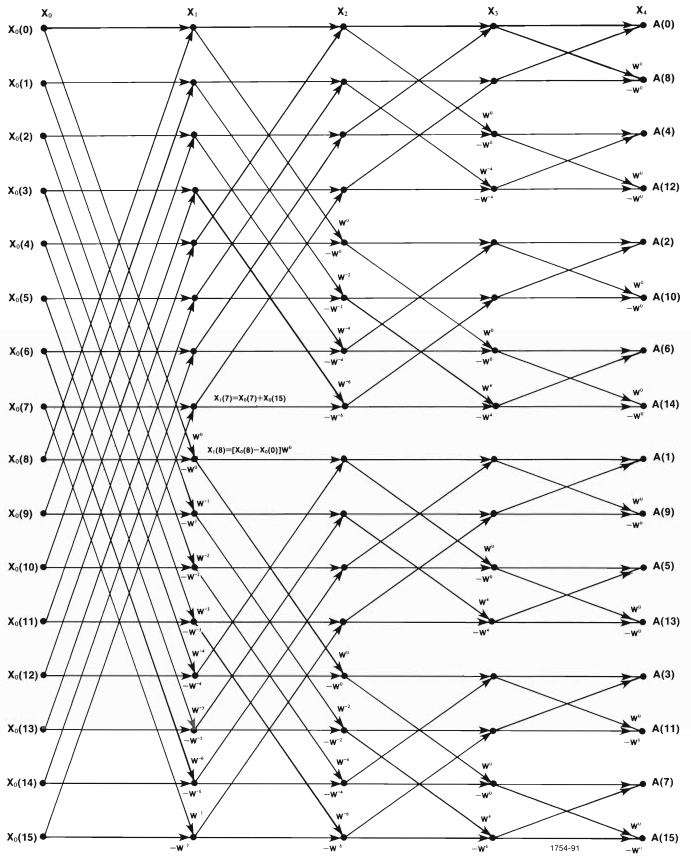
\includegraphics[width=1\textwidth]{images/04/fft.png}
    \end{tabular}
  \end{center}
  \caption{\label{fig:fft} Esquema de uma FFT de um vetor de tamanho 16.}
  \source{Ramirez~\cite{ramirez1975fft}.}
\end{figure}


\clearpage
  
  & O cálculo da FFT consiste de $\log_2 M = K$ estágios. Cada estágio requer pares de cálculos da forma

  \[ f_{k+1}(r) = f_k(r) + f_k(s) \]

  e

  \[ f_{k+1}(s) = (f_k(r) + f_k(s)) W^{-p} \]

  para inteiros $r, s, p$ entre 0 e $M-1$, e para $k$ de 0 a $K$.

  & A Figura~\ref{fig:fft} mostra o esquema do cálculo da FFT de um vetor de tamanho $M = 16$. Cada conjunto de 4 setas saindo de um par $(f_k(r), f_k(s))$ e chegando em um par $(f_{k+1}(r), f_{k+1}(s))$, pelo seu formato, é chamado \textit{butterfly}.

  & A diferença entre $s$ e $r$ diminui com o aumento de $k$ e é dada por $2^{K-k-1}$. Já o expoente $p$ começa sempre como 0 em cada grupo de \textit{butterflies} que se sobrepõem. O incremento do valor de $p$ depende de $k$ e é dado por $2^{k+1}$. A tabela~\ref{tab:fft} mostra os cálculos necessários para obter a FFT de um vetor de tamanho $M = 16$.

\end{easylist}

\begin{table}[!h]
  \centering
  \begin{tabular}{|l|l|l|}
      \hline
      $k=0$ & $k=1$  \\
      $s-r=8$ & $s-r=4$  \\
      $\Delta p = 1$ & $\Delta p = 2$  \\
      \hline
      $f_1(0 ) = (f_0(0 ) + f_0(8 ))      $ & $f_2(0)  = (f_1(0 ) + f_1(4 ))      $  \\
      $f_1(1 ) = (f_0(1 ) + f_0(9 ))      $ & $f_2(1)  = (f_1(1 ) + f_1(5 ))      $  \\
      $f_1(2 ) = (f_0(2 ) + f_0(10))      $ & $f_2(2)  = (f_1(2 ) + f_1(6 ))      $  \\
      $f_1(3 ) = (f_0(3 ) + f_0(11))      $ & $f_2(3)  = (f_1(3 ) + f_1(7 ))      $  \\
      $f_1(4 ) = (f_0(4 ) + f_0(12))      $ & $f_2(4)  = (f_1(0 ) - f_1(4 )) W^{-0}$  \\
      $f_1(5 ) = (f_0(5 ) + f_0(13))      $ & $f_2(5)  = (f_1(1 ) - f_1(5 )) W^{-2}$  \\
      $f_1(6 ) = (f_0(6 ) + f_0(14))      $ & $f_2(6)  = (f_1(2 ) - f_1(6 )) W^{-4}$  \\
      $f_1(7 ) = (f_0(7 ) + f_0(15))      $ & $f_2(7)  = (f_1(3 ) - f_1(7 )) W^{-6}$  \\
      $f_1(8 ) = (f_0(0 ) - f_0(8 )) W^{-0}$ & $f_2(8)  = (f_1(8 ) + f_1(12))       $  \\
      $f_1(9 ) = (f_0(1 ) - f_0(9 )) W^{-1}$ & $f_2(9)  = (f_1(9 ) + f_1(13))       $  \\
      $f_1(10) = (f_0(2 ) - f_0(10)) W^{-2}$ & $f_2(10) = (f_1(10) + f_1(14))       $  \\
      $f_1(11) = (f_0(3 ) - f_0(11)) W^{-3}$ & $f_2(11) = (f_1(11) + f_1(15))       $  \\
      $f_1(12) = (f_0(4 ) - f_0(12)) W^{-4}$ & $f_2(12) = (f_1(8 ) - f_1(12)) W^{-0} $  \\
      $f_1(13) = (f_0(5 ) - f_0(13)) W^{-5}$ & $f_2(13) = (f_1(9 ) - f_1(13)) W^{-2} $  \\
      $f_1(14) = (f_0(6 ) - f_0(14)) W^{-6}$ & $f_2(14) = (f_1(10) - f_1(14)) W^{-4} $  \\
      $f_1(15) = (f_0(7 ) - f_0(15)) W^{-7}$ & $f_2(15) = (f_1(11) - f_1(15)) W^{-6} $  \\
      \hline
      \hline
      $k=2$ & $k=3$  \\
      $s-r=2$ & $s-r=1$  \\
      $\Delta p = 4$ & $\Delta p = 8$  \\
      \hline
      $f_3(0 ) = (f_2(0 ) + f_2(2 ))      $ & $f_4(0 ) = (f_3(0 ) + f_3(1 ))      $  \\
      $f_3(1 ) = (f_2(1 ) + f_2(9 ))      $ & $f_4(1 ) = (f_3(0 ) - f_3(1 )) W^{-0}$  \\
      $f_3(2 ) = (f_2(0 ) - f_2(2 )) W^{-0}$ & $f_4(2 ) = (f_3(2 ) + f_3(3 ))      $  \\
      $f_3(3 ) = (f_2(1 ) - f_2(3 )) W^{-4}$ & $f_4(3 ) = (f_3(2 ) - f_3(3 )) W^{-0}$  \\
      $f_3(4 ) = (f_2(4 ) + f_2(6 ))      $ & $f_4(4 ) = (f_3(4 ) + f_3(5 ))      $  \\
      $f_3(5 ) = (f_0(5 ) + f_0(7 ))      $ & $f_4(5 ) = (f_3(4 ) - f_3(5 )) W^{-0}$  \\
      $f_3(6 ) = (f_2(4 ) - f_2(6 )) W^{-0}$ & $f_4(6 ) = (f_3(6 ) + f_3(7 ))      $  \\
      $f_3(7 ) = (f_2(5 ) - f_2(7 )) W^{-4}$ & $f_4(7 ) = (f_3(6 ) - f_3(7 )) W^{-0}$  \\
      $f_3(8 ) = (f_2(8 ) + f_2(10))      $ & $f_4(8 ) = (f_3(8 ) + f_3(9 ))      $  \\
      $f_3(9 ) = (f_2(9 ) + f_2(11))      $ & $f_4(9 ) = (f_3(8 ) - f_3(9 )) W^{-0}$  \\
      $f_3(10) = (f_2(8 ) - f_2(10)) W^{-0}$ & $f_4(10) = (f_3(10) + f_3(11))      $  \\
      $f_3(11) = (f_2(9 ) - f_2(11)) W^{-4}$ & $f_4(11) = (f_3(10) - f_3(11)) W^{-0}$  \\
      $f_3(12) = (f_2(12) + f_2(14))      $ & $f_4(12) = (f_3(12) + f_3(13))      $  \\
      $f_3(13) = (f_2(13) + f_2(15))      $ & $f_4(13) = (f_3(12) - f_3(13)) W^{-0}$  \\
      $f_3(14) = (f_2(12) - f_2(14)) W^{-0}$ & $f_4(14) = (f_3(14) + f_3(15))      $  \\
      $f_3(15) = (f_2(13) - f_2(15)) W^{-4}$ & $f_4(15) = (f_3(14) - f_3(15)) W^{-0}$  \\
      \hline
  \end{tabular}
  \caption{\label{tab:fft}Etapas do cálculo da FFT de $f$.}
\end{table}

\clearpage

\begin{easylist}

  & Após a execução dos passos descritos, teremos em $f_K$, ou seja, $f_4$ no exemplo, os valores necessários para obter o resultado fora de ordem. É necessário executar a etapa de \textit{bit reversal} para obter o vetor resultante $g$ na ordem correta. Essa etapa consiste em copiar para $g(u)$ o valor de $f_K(R(u))$ onde a operação $R$ denota a reversão dos bits do parâmetro de entrada.
  
\end{easylist}

\begin{table}[!h]
  \centering
  \begin{tabular}{|ccccccc|}
      \hline
      $g(0 )$ & = & $g(0b0000)$ & = & $f_4(0b0000)$ & = & $f_4(0 )$  \\
      $g(1 )$ & = & $g(0b0001)$ & = & $f_4(0b1000)$ & = & $f_4(8 )$  \\
      $g(2 )$ & = & $g(0b0010)$ & = & $f_4(0b0100)$ & = & $f_4(4 )$  \\
      $g(3 )$ & = & $g(0b0011)$ & = & $f_4(0b1100)$ & = & $f_4(12)$  \\
      $g(4 )$ & = & $g(0b0100)$ & = & $f_4(0b0010)$ & = & $f_4(2 )$  \\
      $g(5 )$ & = & $g(0b0101)$ & = & $f_4(0b1010)$ & = & $f_4(10)$  \\
      $g(6 )$ & = & $g(0b0110)$ & = & $f_4(0b0110)$ & = & $f_4(6 )$  \\
      $g(7 )$ & = & $g(0b0111)$ & = & $f_4(0b1110)$ & = & $f_4(14)$  \\
      $g(8 )$ & = & $g(0b1000)$ & = & $f_4(0b0001)$ & = & $f_4(1 )$  \\
      $g(9 )$ & = & $g(0b1001)$ & = & $f_4(0b1001)$ & = & $f_4(9 )$  \\
      $g(10)$ & = & $g(0b1010)$ & = & $f_4(0b0101)$ & = & $f_4(5 )$  \\
      $g(11)$ & = & $g(0b1011)$ & = & $f_4(0b1101)$ & = & $f_4(13)$  \\
      $g(12)$ & = & $g(0b1100)$ & = & $f_4(0b0011)$ & = & $f_4(3 )$  \\
      $g(13)$ & = & $g(0b1101)$ & = & $f_4(0b1011)$ & = & $f_4(11)$  \\
      $g(14)$ & = & $g(0b1110)$ & = & $f_4(0b0111)$ & = & $f_4(7 )$  \\
      $g(15)$ & = & $g(0b1111)$ & = & $f_4(0b1111)$ & = & $f_4(15)$  \\
      \hline
  \end{tabular}
  \caption{\label{tab:bitrev}\textit{Bit reversal} de $f_4$ para obtenção de $g$.}
\end{table}

\begin{easylist}

  & Finalmente, é necessário dividir o vetor $g$ por $M$, para que $g(0)$ seja igual à média de $f$ como convencionado.

  & O algoritmo para o cálculo da inversa, ou seja, da IFFT, é quase idêntico, com duas diferenças. Uma é que não é necessário dividir o resultado por $M$. Também é preciso remover o sinal de menos do expoente de $W^{-p}$, obtendo assim

  \[ f_{k+1}(s) = (f_k(r) + f_k(s)) W^{p} \]


\end{easylist}

  



%%%%%%%%%%%%%%%%%%%%%%%%%%%%%%%%%%%%%%%%%%%%%%%%%%%%%%%%%%%%
%Capítulo: Image enhancement no domínio da frequência
%%%%%%%%%%%%%%%%%%%%%%%%%%%%%%%%%%%%%%%%%%%%%%%%%%%%%%%%%%%%

\chapter{Restauração de imagens}

Capítulo 5 de Gonzalez, \textit{Digital Image Processing}~\cite{gonzalez2006image}.



%%%%%%%%%%%%%%%%%%%%%%%%%%%%%%%%%%%%%%%%%%%%%%%%%%%%%%%%%%%%
%Capítulo: Image enhancement no domínio da frequência
%%%%%%%%%%%%%%%%%%%%%%%%%%%%%%%%%%%%%%%%%%%%%%%%%%%%%%%%%%%%

\chapter{Processamento de imagens coloridas}

Capítulo 6 de Gonzalez, \textit{Digital Image Processing}~\cite{gonzalez2006image}.

\vspace{.5cm}

\begin{easylist}

  & O processamento de imagens coloridas pode ser dividido em duas grandes áreas:
  && Processamento de imagens em \textit{full-color}.
  && Processamento de imagens em cor falsa.

\end{easylist}
  
%%%%%%%%%%%%%%%%%%%%%%%%%%%%%%%%%%%%%%%%%%%%%%%%%%%%%%%%%%%%
\section{Fundamentos de teoria de cor}

\begin{easylist}

  & Percepção e interpretação: a forma como percebemos e interpretamos cores é regida por fenômenos psicofisiológicos, que envolvem estímulos dos sensores da retina e pulsos elétricos nos nervos e no córtex visual. A percepção de uma cor pode variar entre pessoas diferentes mas é determinada principalmente pela natureza da luz emitida ou refletida por um objeto.

  & Caracterização da luz: três medidas podem ser usadas para caracterizar uma fonte de luz:
  && Radiância: energia que flui de uma fonte de luz, normalmente medida em watts (W).
  && Luminância: energia que pode ser vista por um observador, medida em lumens (lm). Uma fonte de luz infravermelha pode ter muita radiância, mas terá luminância praticamente nula.
  && Brilho ou intensidade: descritor subjetivo que indica o quanto uma fonte de luz parece próxima ao branco. Uma fonte de luz verde ou amarela parece mais brilhante que uma azul ou vermelha. A Figura~\ref{fig:bright} mostra um exemplo de padrão de teste com barra de cores com os valores das cores antes e depois de a imagem ser convertida para escala de cinza. Observe como as cores mais brilhantes em~\ref{fig:bright:rgb} possuem valores maiores de brilho em~\ref{fig:bright:gray}.


  \begin{figure}[!t]
  \begin{subfigure}{1\textwidth}
    \centering
    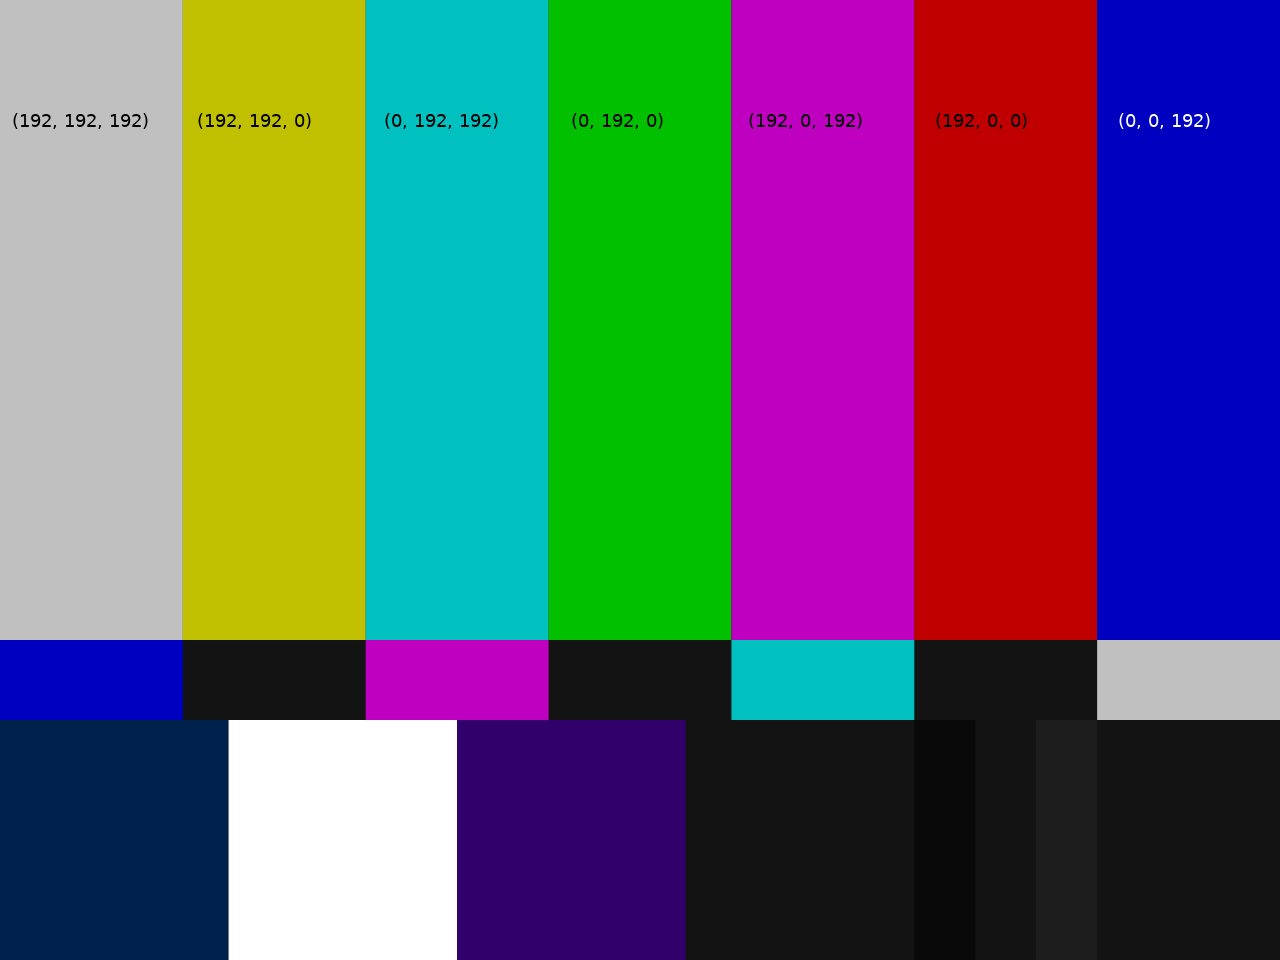
\includegraphics[width=0.75\textwidth]{images/06/SMPTE_Color_Bars_RGB.png}
    \caption{\label{fig:bright:rgb} Exemplos de cores RGB}
  \end{subfigure}
  \begin{subfigure}{1\textwidth}
    \centering
    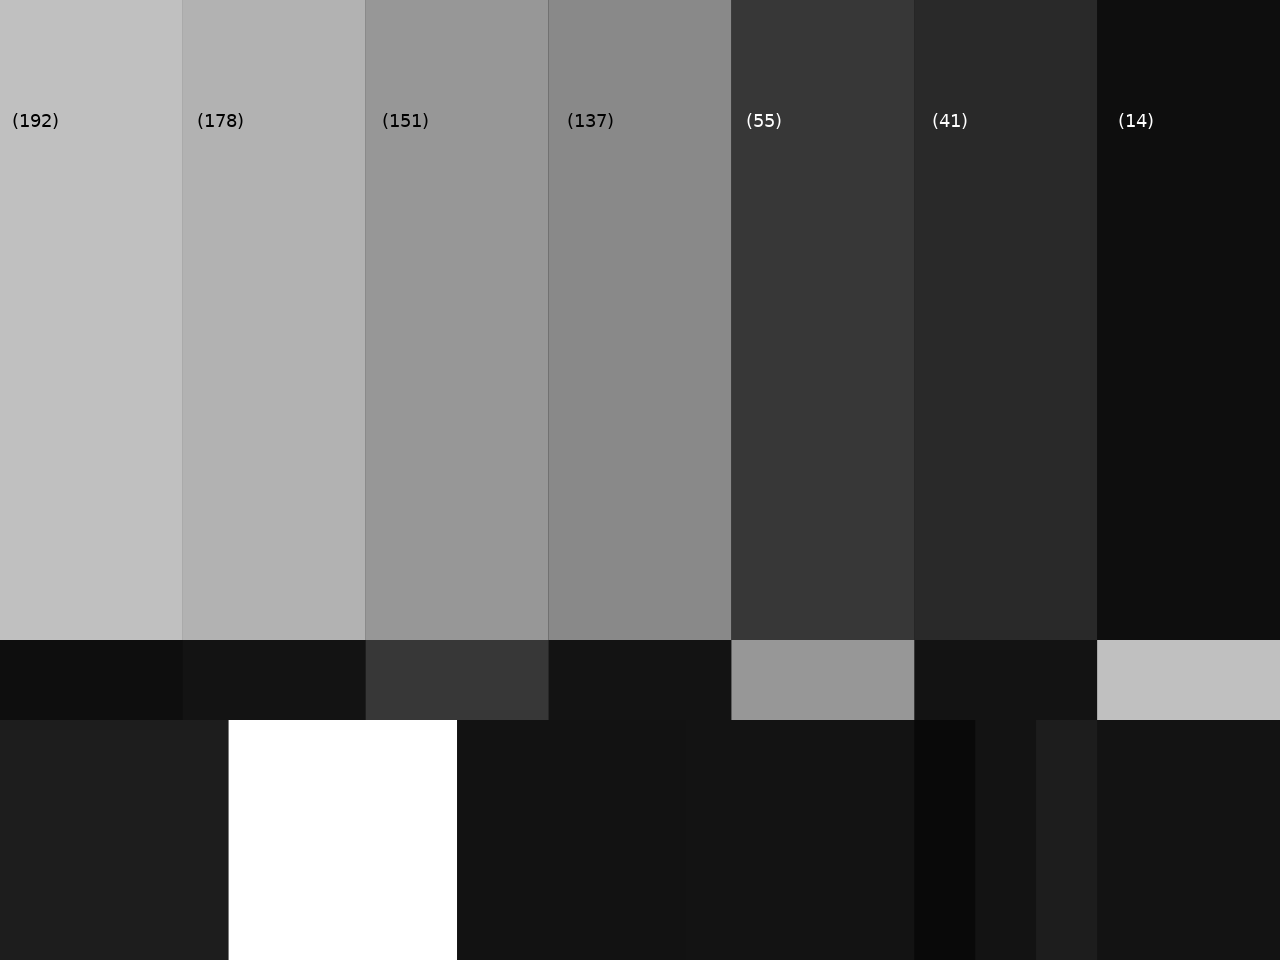
\includegraphics[width=0.75\textwidth]{images/06/SMPTE_Color_Bars_gray.png}
    \caption{\label{fig:bright:gray} Versão em escala de cinza com valores das intensidades.}
  \end{subfigure}
  \caption{\label{fig:bright} Padrão de teste com barras de cores.}
  \source{Adaptado de \tt{https://en.wikipedia.org/wiki/SMPTE\UL color\UL bars}.}
  \end{figure}


  


  
  \vspace{.5cm}

  & Outra maneira de caracterizar uma fonte de luz é quanto à presença ou ausência de cor:

  && Luz acromática: é a luz sem cor. Sua única característica é a intensidade. Uma fonte de luz com todas ou algumas cores do espectro de maneira equilibrada, parecerá acromática. O termo ``tom de cinza'' se refere a uma medida escalar de intensidade que vai do preto ao branco, passando pelas diversas tonalidades de cinza.
  && Luz cromática: é a luz com cor, seja ela monocromática ou composta por vários comprimentos de onda de maneira que não pareça branca. Pode ser caracterizada pelo seu brilho, matiz e saturação. O brilho indica a noção acromática de intensidade. O matiz indica o comprimento de onda dominante, e a saturação indica se a luz é pura ou se está misturada com luz branca. As cores do espectro têm saturação máxima. As cores misturadas com branco têm pouca saturação.
  && Cromaticidade: é uma medida que une o matiz e a saturação. Portanto, uma cor pode ser caracterizada pelo seu brilho e pela sua cromaticidade. A cromaticidade é dada pela quantidade de vermelho, verde e azul que formam uma cor, e sua soma é sempre 1. 

\end{easylist}

\[ r = \frac{R}{R+G+B}
   \hspace{1.1cm}
   g = \frac{G}{R+G+B}
   \hspace{1.1cm}
   b = \frac{B}{R+G+B}
   \]

\begin{figure}[!h]
  \begin{center}
    \begin{tabular}{c}
      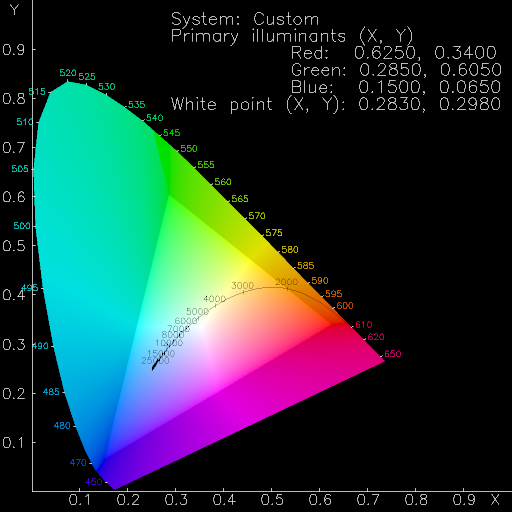
\includegraphics[width=0.7\textwidth]{images/06/chromaticity.png}
    \end{tabular}
  \end{center}
  \caption{\label{fig:chromaticity} Diagrama de cromaticidade de um certo dispositivo.}
  \source{\tt{http://www.libpng.org}.}
\end{figure}

   
%%%%%%%%%%%%%%%%%%%%%%%%%%%%%%%%%%%%%%%%%%%%%%%%%%%%%%%%%%%%
\section{Modelos de cor}

\begin{easylist}

  & Modelos de cor, também conhecidos como espaços de cor ou sistemas de cor, servem para especificar cores de maneira padronizada. É uma especificação de um sistema de coordenadas e de uma região desse espaço onde cada cor é representada por um único ponto. Geralmente, a especificação de um modelo de cor é feita para suportar algum tipo de hardware ou aplicação.

  & Tipos de modelos de cor
  && Modelos aditivos: a soma dos componentes dá branco.
  && Modelos subtrativos: a soma dos componentes dá preto.


  & Exemplos de modelos de cor
  && RGB: modelo usado para representar imagens digitais a serem exibidas em monitores. É um modelo aditivo. Consiste de três componentes: $R$, $G$ e $B$. O espaço de cor RGB costuma ser representado por um cubo de lado igual a 1. Digitalmente, cada dimensão do cubo costuma ser representada por valores de 8 bits. Dessa forma, cada pixel possui profundidade de 24 bits. Valores maiores de bits podem ser usados, caso em que temos uma imagem HDR (\textit{High Dynamic Range}). A diagonal do cubo entre os pontos $(0,0,0)$ e $(1,1,1)$ representa as escalas de cinza. O cubo completo, se representado por valores de 24 bits, é composto por $2^{24}$ cores.

\end{easylist}

  \begin{figure}[!h]
  \begin{center}
    \begin{tabular}{c}
      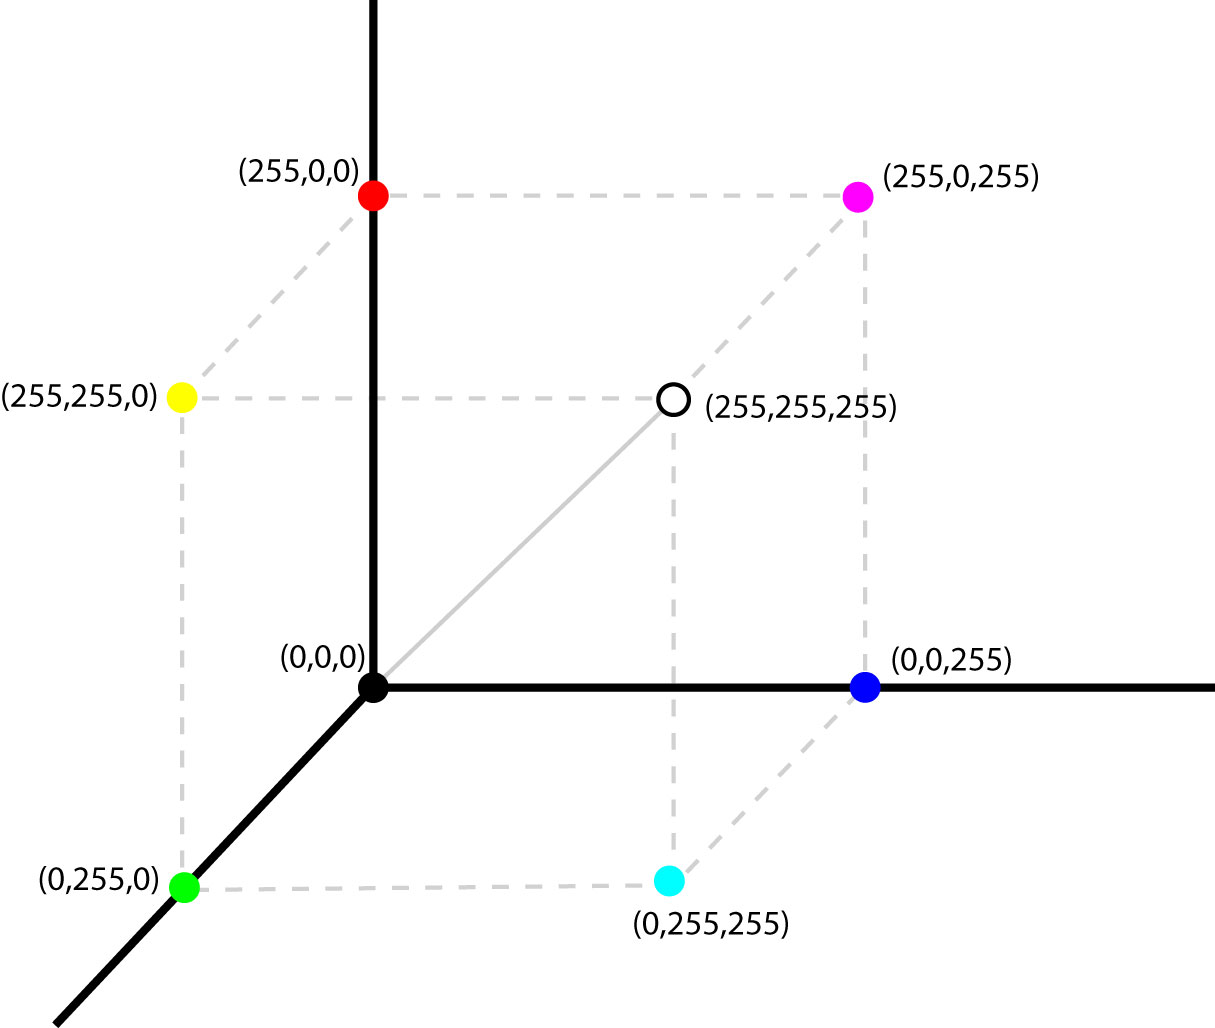
\includegraphics[width=0.5\textwidth]{images/06/RGB_cube.jpg}
    \end{tabular}
  \end{center}
  \caption{\label{fig:rgb} Espaço de cor RGB.}
  \source{\tt{http://commons.wikimedia.org}.}
\end{figure}
  
\begin{easylist}
  
  && CMY e CMYK: modelo usado por dispositivos de impressão. É um modelo subtrativo. A conversão de RGB para CMY pode ser feita através da operação:

\end{easylist}


  \[
    \begin{bmatrix}
      C \\ M \\ Y \\
    \end{bmatrix}  
    =
    \begin{bmatrix}
      1 \\ 1 \\ 1 \\
    \end{bmatrix}  
    -
    \begin{bmatrix}
      R \\ G \\ B \\
    \end{bmatrix}  
  \]

\begin{easylist}

  A cor preta é adicionada por diversas razões:

  &&& Uma impressão precisa de texto seria muito difícil sem a cor preta, pois exigiria o registro preciso dos três canais.
  &&& A composição do preto com as três cores é mais cara, requer mais tinta, pode ensopar o papel, pode demorar a secar, pode borrar a imressão, e a aparência é de uma cor escura, mas não exatamente da cor preta.

\end{easylist}



%%%%%%%%%%%%%%%%%%%%%%%%%%%%%%%%%%%%%%%%%%%%%%%%%%%%%%%%%%%%
%Capítulo: Processamento morfológico de imagens
%%%%%%%%%%%%%%%%%%%%%%%%%%%%%%%%%%%%%%%%%%%%%%%%%%%%%%%%%%%%

\chapter{Processamento morfológico de imagens}

Capítulo 9 de Gonzalez, \textit{Digital Image Processing}~\cite{gonzalez2006image}.


%%%%%%%%%%%%%%%%%%%%%%%%%%%%%%%%%%%%%%%%%%%%%%%%%%%%%%%%%%%%
\section{Introdução}

\begin{easylist}

  & Morfologia Matemática denota um conjunto de ferramentas úteis para representar e descrever formas de regiões da imagem, como bordas, esqueletos e casco convexo. Também são úteis como operações de pré e pós-processamento, como filtragem morfológica e afinamento.
  
  & Duas operações fundamentais da Morfologia Matemática são erosão e dilatação.

\end{easylist}


%%%%%%%%%%%%%%%%%%%%%%%%%%%%%%%%%%%%%%%%%%%%%%%%%%%%%%%%%%%%
\section{Erosão e dilatação}

\begin{easylist}

  & Erosão: seja $f$ uma imagem digital em escala de cinza e $S$ um conjunto de pixels centrado na origem. Denotamos erosão por

  \[ (f \ominus S)(x) = \min\{ f(x+z) | z \in S \} \]

  onde $S$ é conhecido como elemento estruturante e $x$ são as coordenadas dos pixels de $f$.
  
  & Dilatação: seja $f$ uma imagem digital em escala de cinza e $S$ um conjunto de pixels centrado na origem. Denotamos dilatação por

  \[ (f \oplus S)(x) = \max\{ f(x-z) | z \in S \} \]

  onde $S$ é conhecido como elemento estruturante e $x$ são as coordenadas dos pixels de $f$.

  & Dualidade: a erosão e dilatação são duais um do outro com relação ao complemento e reflexão do elemento estruturante na medida em que

  \[ (f \ominus S)^c = f^c \oplus \hat{S} \]

ou 
  
  \[ (f \oplus S)^c = f^c \ominus \hat{S} \]

  onde o $c$ superescrito denota o complementar de imagens binárias ou a negativa de imagens em escala de cinza, e $\hat{S}$ denota a reflexão do elemento estruturante $S$ em relação à origem. Algumas implementações da dilatação e erosão podem não preservar a dualidade a depender de suas especificidades.

\end{easylist}


%%%%%%%%%%%%%%%%%%%%%%%%%%%%%%%%%%%%%%%%%%%%%%%%%%%%%%%%%%%%
\section{Abertura e fechamento}

\begin{easylist}

  & Abertura de $f$ pelo elemento estruturante $S$ é denotada por $f \circ S$ e é definida por

  \[ f \circ S = (f \ominus S) \oplus S. \]

  & Fechamento de $f$ pelo elemento estruturante $S$ é denotada por $f \bullet S$ e é definida por

  \[ f \bullet S = (f \oplus S) \ominus S. \]

\end{easylist}


%%%%%%%%%%%%%%%%%%%%%%%%%%%%%%%%%%%%%%%%%%%%%%%%%%%%%%%%%%%%
\section{Operador \textit{hit-miss}}

\begin{easylist}

  & O operador \textit{hit-miss} é um operador usado para detecção de formas (\textit{shape detection}). O elemento estruturante usado pode conter, além dos valores 0 e 1, o valor X, ou \textit{don't care}. O elemento estruturante

  \end{easylist}

  \[
    B = 
    \begin{bmatrix}
      X & 0 & 0 \\
      1 & 1 & 0 \\
      X & 1 & X \\
    \end{bmatrix}  
  \]
    
\begin{easylist}

  e suas rotações por múltiplos de $90^\circ$ pode ser usado para detectar cantos. Seu complemento, necessário no processo, é

\end{easylist}
  
  \[
    B = 
    \begin{bmatrix}
      X & 1 & 1 \\
      0 & 0 & 1 \\
      X & 0 & X \\
    \end{bmatrix}  
  \]

\begin{easylist}

  & O operador \textit{hit-miss} pelo elemento estruturante $B$ da imagem $f$ é denotado por $f \circledast B$ e é dado por

  \[ f \circledast B = (f \ominus B) \cap (f^c \ominus B^c). \]

  & Considere que $B_\alpha$ é o elemento estruturante $B$ rotacionado pelo ângulo $\alpha$ no sentido anti-horário. Poderíamos obter todos os cantos da imagem através da operação abaixo.

  \[ (f \circledast B_{0})  \cup
     (f \circledast B_{90}) \cup
     (f \circledast B_{180}) \cup
     (f \circledast B_{270})      \]

\end{easylist}


%%%%%%%%%%%%%%%%%%%%%%%%%%%%%%%%%%%%%%%%%%%%%%%%%%%%%%%%%%%%
\section{Algoritmos morfológicos básicos}

\begin{easylist}

  & Extração de borda: a borda de uma imagem f, denotada por $\beta(f)$, pode ser obtida por uma erosão de $f$ pelo elemento estruturante $B$, e depois fazendo a diferença entre $f$ e sua erosão, ou seja,

  \[ \beta(f) = f - (f \ominus B). \]

  São alternativas a esse operador  

  \[ \beta_d(f) = (f \oplus B) - f \]

  e

  \[ \beta_c(f) = (f \oplus B) - (f \ominus B). \]

  & Preenchimento de buracos: Seja $A$ um conjunto de pixels com valor 1 4-conectados ao redor de uma região de pixels com valor 0, ou seja, um buraco. Seja $p$ um pixel pertencente ao buraco. Nosso objetivo é preencher o buraco inteiro com pixels valor 1. O procedimento a seguir preenche o buraco:

  \medskip
  \hspace{1cm}    \textit{do}
  
  \hspace{1cm}\hspace{1cm}    $X_k = (X_{k-1} \oplus B) \cap A^c, k = 1, 2, 3\dots$

  \hspace{1cm}    \textit{while} $X_k \neq X_{k-1}$
  \medskip

  onde $X_0 = p$ e $B$ é o quadrado $3\times3$. Ao final, a união de $X_k$ e $A$ nos dá a região preenchida.

  & Extração de componentes conexos: Seja $Y \subseteq A$ um componente conexo, e $p \in Y$ um pixel. O procedimento a seguir nos dá todos os pontos de $Y$:

  \medskip
  \hspace{1cm}    \textit{do}
  
  \hspace{1cm}\hspace{1cm}    $X_k = (X_{k-1} \oplus B) \cap A, k = 1, 2, 3\dots$

  \hspace{1cm}    \textit{while} $X_k \neq X_{k-1}$
  \medskip

  onde $X_0 = p$ e $B$ é um elemento estruturante adequado.  

\clearpage
  
  & Rotulação de componentes conexos em imagens binárias: o processo de rotulação consiste em preencher com uma cor ou rótulo diferente cada um dos componentes conexos de uma imagem. O rótulo 0 é reservado para o \textit{background}. O algoritmo abaixo pode ser usado nesse processo. Recebe como entrada uma imagem binária cujos pixels têm valores no conjunto ${0, 255}$.

  \medskip
  \ind label = 1
  
  \ind \textit{foreach} pixel p
  
  \ind \ind \textit{if} value(p) == 255
  
  \ind \ind \ind value(p) = label

  \ind \ind \ind Q.enqueue(p)

  \ind \ind \ind \textit{while} !Q.empty()

  \ind \ind \ind \ind c = Q.dequeue()

  \ind \ind \ind \ind \textit{foreach} d = neighbor(c)

  \ind \ind \ind \ind \ind \textit{if} value(d) == 255

  \ind \ind \ind \ind \ind \ind value(d) == label
  
  \ind \ind \ind \ind \ind \ind Q.enqueue(d)

  \ind \ind \ind label++
  
  \medskip
  
\end{easylist}



%%%%%%%%%%%%%%%%%%%%%%%%%%%%%%%%%%%%%%%%%%%%%%%%%%%%%%%%%%%%
%Capítulo: Entrada e saída
%%%%%%%%%%%%%%%%%%%%%%%%%%%%%%%%%%%%%%%%%%%%%%%%%%%%%%%%%%%%

%\input{io.tex}


%%%%%%%%%%%%%%%%%%%%%%%%%%%%%%%%%%%%%%%%%%%%%%%%%%%%%%%%%%%%
%Capítulo: Vetores
%%%%%%%%%%%%%%%%%%%%%%%%%%%%%%%%%%%%%%%%%%%%%%%%%%%%%%%%%%%%

%\input{array.tex}


%%%%%%%%%%%%%%%%%%%%%%%%%%%%%%%%%%%%%%%%%%%%%%%%%%%%%%%%%%%%
%Capítulo: Funções
%%%%%%%%%%%%%%%%%%%%%%%%%%%%%%%%%%%%%%%%%%%%%%%%%%%%%%%%%%%%

%\input{function.tex}


%%%%%%%%%%%%%%%%%%%%%%%%%%%%%%%%%%%%%%%%%%%%%%%%%%%%%%%%%%%%
%Capítulo: Exercícios
%%%%%%%%%%%%%%%%%%%%%%%%%%%%%%%%%%%%%%%%%%%%%%%%%%%%%%%%%%%%

%\input{exercise.tex}




%%%%%%%%%%%%%%%%%%%%%%%%%%%%%%%%%%%%%%%%%%%%%%%%%%%%%%%%%%%%
%Capítulo: Exemplos de programas
%%%%%%%%%%%%%%%%%%%%%%%%%%%%%%%%%%%%%%%%%%%%%%%%%%%%%%%%%%%%

%\chapter{Exemplos de programas}


%%%%%%%%%%%%%%%%%%%%%%%%%%%%%%%%%%%%%%%%%%%%%%%%%%%%%%%%%%%%
%Seção: pause.cpp

%\section{pause.cpp}

%\lstinputlisting[caption=series.cpp]{src/pause.cpp}

%%%%%%%%%%%%%%%%%%%%%%%%%%%%%%%%%%%%%%%%%%%%%%%%%%%%%%%%%%%%
%Seção: ascii.cpp

%\section{ascii.cpp}

%\lstinputlisting[caption=ascii.cpp]{src/ascii.cpp}

%%%%%%%%%%%%%%%%%%%%%%%%%%%%%%%%%%%%%%%%%%%%%%%%%%%%%%%%%%%%
%Seção: dado.cpp

%\section{dado.cpp}

%\lstinputlisting[caption=dado.cpp]{src/dado.cpp}

%%%%%%%%%%%%%%%%%%%%%%%%%%%%%%%%%%%%%%%%%%%%%%%%%%%%%%%%%%%%
%Seção: primos.cpp

%\section{primos.cpp}

%\lstinputlisting[caption=series.cpp]{src/primos.cpp}

%%%%%%%%%%%%%%%%%%%%%%%%%%%%%%%%%%%%%%%%%%%%%%%%%%%%%%%%%%%%
%Seção: series.cpp

%\section{series.cpp}

%\lstinputlisting[caption=series.cpp]{src/series.cpp}




%%%%%%%%%%%%%%%%%%%%%%%%%%%%%%%%%%%%%%%%%%%%%%%%%%%%%%%%%%%%
%Seção: generate.cpp

%\section{generate.cpp}

%\lstinputlisting[caption=generate.cpp]{src/generate.cpp}

%%%%%%%%%%%%%%%%%%%%%%%%%%%%%%%%%%%%%%%%%%%%%%%%%%%%%%%%%%%%
%Seção: ordena.cpp

%\section{ordena.cpp}

%\lstinputlisting[caption=ordena.cpp]{src/ordena.cpp}

\nocite{gonzalez2006image,
dougherty2003handson,
learning_opencv,
Duda:2001,
Costa:2001,
Jain1995machine,
soille1999morphological,
Tufte:83,
GeometryMultiple,
MultipleView,
3dComputer}

\bibliography{refs}
\bibliographystyle{plain}


\end{document}

